\documentclass[12pt,a4paper]{article}
\title{Spinach Stir Fry}
\author{}
\date{}
\usepackage{graphicx}
\begin{document}
\maketitle

\begin{figure}[t]
    \centering
    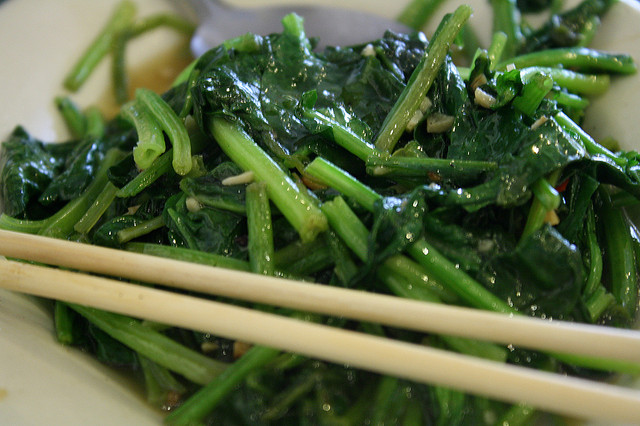
\includegraphics[scale=0.5]{stirfryspinach.jpg}
\end{figure}
\section*{Details}
\begin{itemize}
    \item Prep time - under 10 mins
    \item Cook time - Under 20 mins
    \item Serves - 3
\end{itemize}


\section*{Ingredients needed}
\begin{itemize}
    \item Spinach - 1 bunch or 3 cups tightly packed 
    \item Pearl onions/ small onions - 1/4 cup
    \item Garlic cloves- 4 (optional)
    \item Grated Coconut - 2 1/2 tbsp
\end{itemize}

\section*{For the seasoning}
\begin{itemize}
    \item Oil - 1 tbsp
    \item Mustard seeds- 1 tsp
    \item Split urad dal - 3/4 tsp
    \item Red Chilli - 3 (broken into 2 pieces)
\end{itemize}

\section*{Preparation}

\begin{enumerate}
    \item Clean and wash greens well. Chop it finely and keep it aside.
    \item Chop pearl onions and garlic finely 
    \item Heat oil, add mustard seeds, when it splutters, add urad dal and red chillies.
    \item Saute for a few seconds, add finely chopped onions and garlic.
    \item Saute till onions turn transparent. Add the chopped greens and stir well.
    \item Keep the flames low and cook covered. Add salt after the greens wilt.
    \item Stir in between and sprinkle water only if required.
    \item Once the greens are cooked, add grated coconut and mix well. Switch off the flame and serve hot.
\end{enumerate}
\section*{Variations}

If you like cumin flavour, crush 1/2 tsp cumin seeds along with grated coconut and mix it with the greens before switching off the flame.

\end{document}

